%! Author = fabian
%! Date = 21.11.21

% Preamble
\documentclass[a4paper]{article} % Uses article class in A4 format

%----------------------------------------------------------------------------------------
%	FORMATTING
%----------------------------------------------------------------------------------------

\addtolength{\hoffset}{-2.25cm}
\addtolength{\textwidth}{4.5cm}
\addtolength{\voffset}{-3.25cm}
\addtolength{\textheight}{5cm}
\setlength{\parskip}{0pt}
\setlength{\parindent}{0in}


%----------------------------------------------------------------------------------------
%	PACKAGES AND OTHER DOCUMENT CONFIGURATIONS
%----------------------------------------------------------------------------------------

\usepackage[utf8]{inputenc} % Use UTF-8 encoding
%\usepackage{microtype} % Slightly tweak font spacing for aesthetics

\usepackage[english]{babel} % Language hyphenation and typographical rules

\usepackage{amsthm, amsmath, amssymb, bm} % Mathematical typesetting
\usepackage{float} % Improved interface for floating objects
%\usepackage[final, colorlinks = true,
%linkcolor = black,
%citecolor = black]{hyperref} % For hyperlinks in the PDF
\usepackage{graphicx, multicol} % Enhanced support for graphics
\usepackage{caption}
\usepackage{subcaption}
\usepackage{xcolor} % Driver-independent color extensions
%\usepackage{marvosym, wasysym} % More symbols
%\usepackage{rotating} % Rotation tools
%\usepackage{censor} % Facilities for controlling restricted text!
%\usepackage{booktabs} % Enhances quality of tables
%\usepackage{censor} % Facilities for controlling restricted text!
%\usepackage{booktabs} % Enhances quality of tables
\usepackage{listings}
\usepackage{enumitem}


%\usepackage{csquotes} % Context sensitive quotation facilities
\usepackage[yyyymmdd]{datetime} % Uses YEAR-MONTH-DAY format for dates
\renewcommand{\dateseparator}{-} % Sets dateseparator to '-'

\usepackage{fancyhdr}
\usepackage{amsmath}
\usepackage{bm}
\usepackage{amsfonts} % Headers and footers
\pagestyle{fancy} % All pages have headers and footers
\fancyhead{}\renewcommand{\headrulewidth}{0pt} % Blank out the default header
\fancyfoot[L]{} % Custom footer text
\fancyfoot[C]{} % Custom footer text
\fancyfoot[R]{\thepage} % Custom footer text

%\newcommand{\note}[1]{\marginpar{\scriptsize \textcolor{red}{#1}}} % Enables comments in red on margin
\DeclareMathOperator*{\argmax}{argmax}
\DeclareMathOperator*{\argmin}{argmin}
%----------------------------------------------------------------------------------------

% Document
\begin{document}
%----------------------------------------------------------------------------------------

%	TITLE SECTION
    \title{Title} % Article title
    \fancyhead[C]{}
    \hrule \medskip % Upper rule
    \begin{minipage}{0.295\textwidth} % Left side of title section
        \raggedright
        TTK4255\\ % Your lecture or course
        \footnotesize % Authors text size
        \hfill\\
        Fabian Höldin \\
        Sindre {\O}versveen% Your name, your matriculation number
    \end{minipage}
    \begin{minipage}{0.4\textwidth} % Center of title section
        \centering
        \large % Title text size
        Robotic Vision \\ % Assignment title and number
        \normalsize % Subtitle text size
        Midterm project:\\
        Model-based pose estimation\\ % Assignment subtitle
    \end{minipage}
    \begin{minipage}{0.295\textwidth} % Right side of title section
        \raggedleft
        \today\\ % Date
        \footnotesize % Email text size
        \hfill\\
        % Your email
    \end{minipage}
    \medskip\hrule % Lower rule
%----------------------------------------------------------------------------------------
%	ARTICLE CONTENTS
%----------------------------------------------------------------------------------------

\section{Estimate the helicopter angles}
    \subsection*{Task 1.1}
    \begin{figure*}[h]
        \centering
        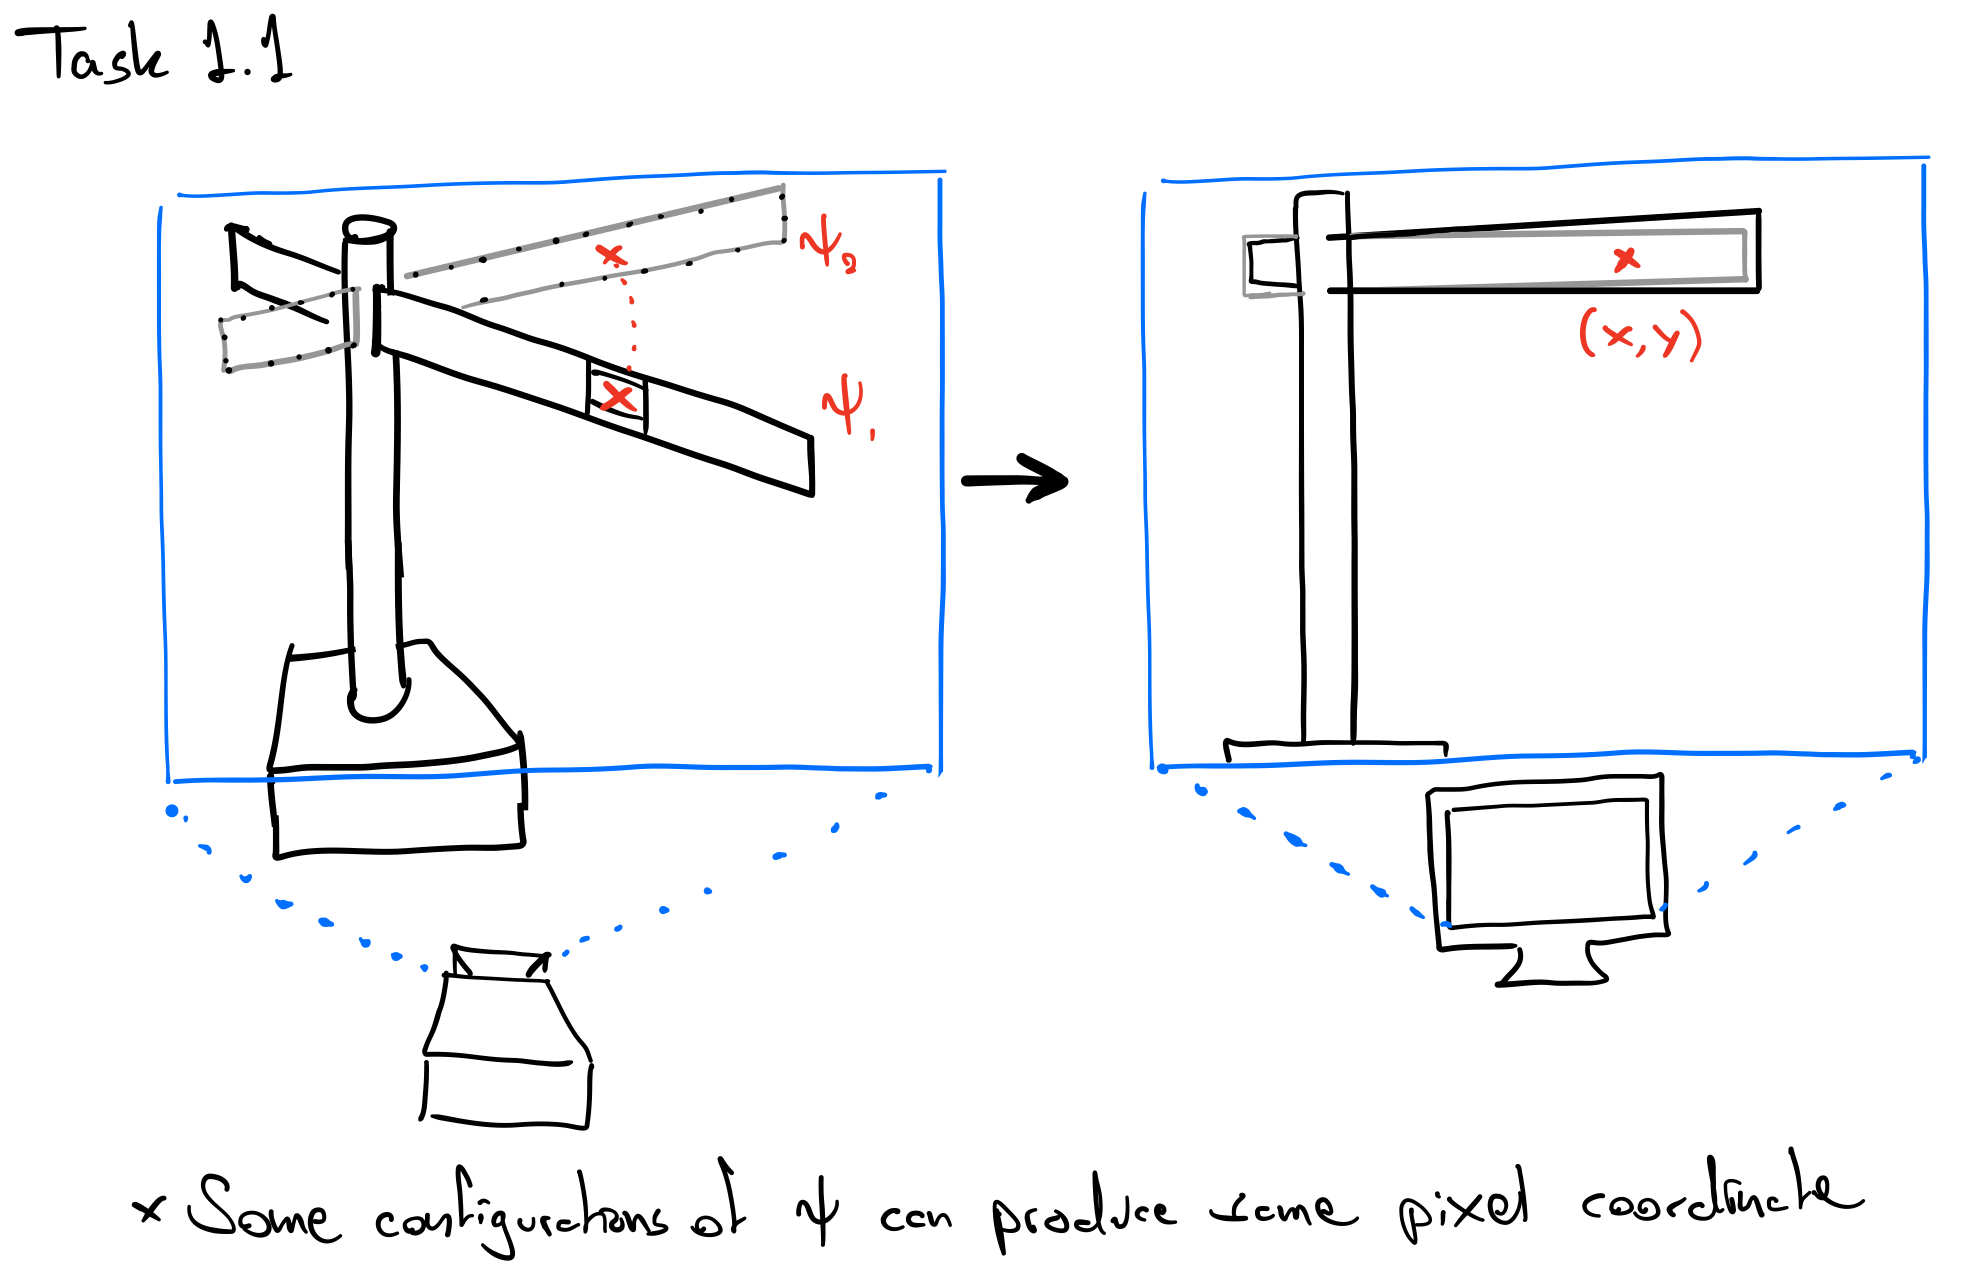
\includegraphics[width= 0.7 \linewidth]{../python/Task1.1_Sketch}
        \caption{Projection into camera plane}
    \end{figure*}
    As you can see in the above sketch, two points from the 3D world coordinate system can correspond to one in the camera view.
    This is due to the loss of one dimension (depth), what makes it impossible to distinguish single points that only differ in their distance to the camera.

    \subsection*{Task 1.2}
    The linearization of absolute values is probably much less efficient.
    Calculating horizontal and vertical differences is a very trivial task and preserves the uniqueness of configurations (+-u,v).

    \subsection*{Task 1.3}
    Optimal angles (residuals) on image 0:
    \begin{center}
        \begin{tabular}{ccccccc}
            5.24245604 & 4.80020124 & 1.19885845 & -4.99317996 & -4.47286417 & 0 & 0.04965743 \\
            -8.87519959 & -5.02385631 & -6.06002405 & -2.97156827 & 0.43079638 & 0 & -6.26710301
        \end{tabular}
    \end{center}
    \begin{figure*}[h]
        \centering
        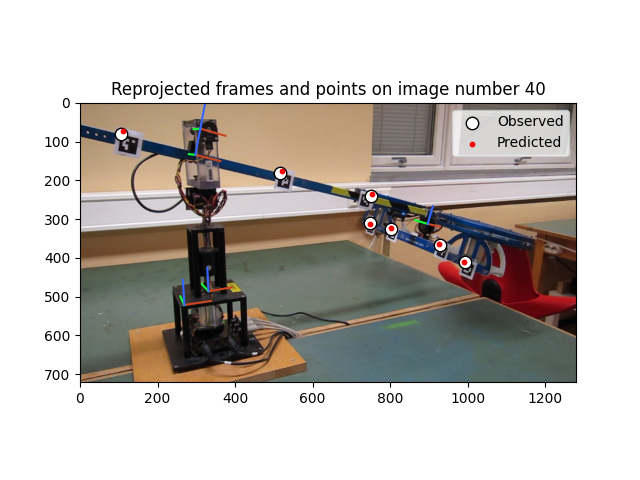
\includegraphics[width= 0.7 \linewidth]{../python/out_part1a_10steps}
    \end{figure*}
    Reprojection errors at solution:\\
    Marker 1: 10.60 px\\
    Marker 2:  7.26 px\\
    Marker 3:  5.06 px\\
    Marker 4:  2.70 px\\
    Marker 5:  1.85 px\\
    Marker 6:  3.57 px\\
    Marker 7:  1.90 px\\
    Average:   4.71 px\\
    Median:    3.57 px

    \subsection*{Task 1.4}
    \begin{center}
        \begin{tabular}{cccc}
            \hline
            $\bm{p_0}$ & steps & Avg.Err. & Med.Err \\
            \hline \hline
            $ \bigl[ \begin{smallmatrix}
                         0.0 & 0.0 & 0.0
            \end{smallmatrix} \bigr] ^T$ &
            3 & 4.71 px & 3.38 px\\
            $ \bigl[ \begin{smallmatrix}
                         0.5 & 0.5 & 0.5
            \end{smallmatrix} \bigr] ^T$ &
            3 & 4.71 px & 3.61 px \\
            $ \bigl[ \begin{smallmatrix}
                         1.0 & 1.0 & 1.0
            \end{smallmatrix} \bigr] ^T$ &
            4 & 4.71 px & 3.80 px\\
        \end{tabular}
    \end{center}
    As can be seen in the above table, the initial value $\bm{p_0}$ does not change the amount of steps nor the reprojection error significantly.

    \subsection*{Task 1.5}
    We get this warning because we are trying to solve an under-determined system of linear equations what results in having infinite many solutions.
    The "numpy.linalg.solve()" function cannot handle this.

    \subsection*{Task 1.6}
    For simply extending the dimensions $\bm{p} \in \mathbb{R}^4$ we will get a Jacobian $ \bm{J} \in \mathbb{R}^{n \times 4}$ and an approximate Hessian $\bm{J}^T \bm{J} \in \mathbb{R}^{4 \times 4} $.
    The modification of the helicopter model might result in not having unique configurations for one specific model state, e.g. $\phi$ and $\psi$ are nearly indistinguishable for straight upwards pointing helicopter.

    \subsection*{Task 1.7}
    \begin{enumerate}[label=(\alph*)]
        \item The maximum error is 19.4877 pixels.
        \item This maximum error occurs in image 104.
        The minimum error occurs in image 152.
        \item Parameter : \\
        - Yaw: max = 0.7999 , image: 187 \\
        - Pitch: max = 0.2431, image: 327 \\
        - Roll: max = 0.0748, image: 350 \\
        The minimum errors are 0 at image 0 because of the offset synchronization we use.
    \end{enumerate}

    \subsection*{Task 1.8}
    \begin{enumerate}[label=(\alph*)]
        \item Because of the way the residue function has been implemented, with the weights for valid entries, the residue of unobserved markers are set to zero.
            Followingly, the corresponding index of the jacobian matrix $J$ will be zero too - leading to a potentially singular matrix, which prevents solving for a unique solution.
            The Levenberg-Marquardt method has circumvented this problem by fixing the step length to 1 and adding a term $\mu*I$ to the normal equation.
            This guarantees that the equation remains solvable and that the estimation algorithm can move past the points with insufficient observational data.
        \item The added term $\mu I$ adds $\mu 1$ to the diagonal elements of $J^TJ$, with \mu having a variable magnitude.
            The Levenberg-Marquardt method is set up in such a way that the $\mu$ term decreases when approaching the minimum, and increases otherwise.
            This means that the $J^TJ$ term will dominate when close to the minimum, leveraging the benefits of Newton-Gauss, while having the '+1' term dominate further from the minimum - where Newton-Gauss struggles.
            The downside of this method, is the fixed step length of 1.
            While Levenberg-Marquardt is robust in ensuring that each step of the optimization remains solvable, it suffers from a sort of 'maximum accuracy' - with no guarantees beyond 'minimum + 1'.
            This must be taken into account when determining the stopping criterion.
    \end{enumerate}

\section{Estimate the platform pose}
    \subsection*{Task 2.1}
    \begin{figure}[h]
        \centering
        \begin{subfigure}{0.45\textwidth}
            \centering
            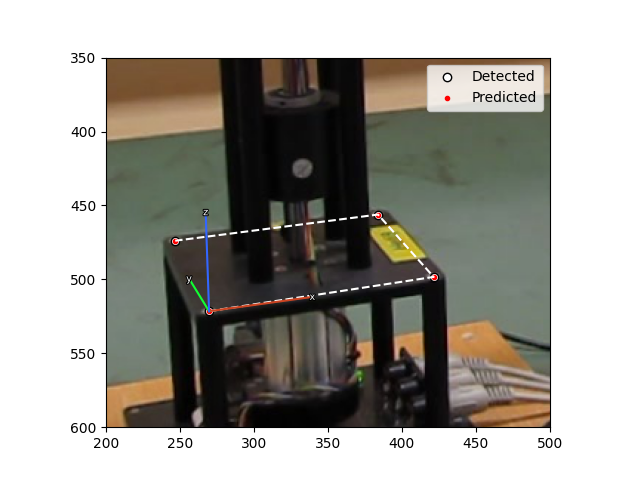
\includegraphics[width= \textwidth]{../python/out_part2_1a}
            \caption{Output equation $\bm{\tilde{u}} = \bm{KH}
                \begin{bmatrix}
                    X & Y & 1
                \end{bmatrix}
            ^T$ }

        \end{subfigure}
        \hfill
        \begin{subfigure}{0.45\textwidth}
            \centering
            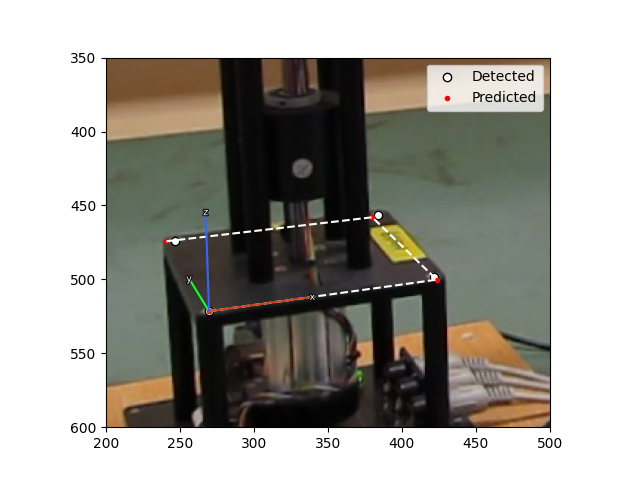
\includegraphics[width= \textwidth]{../python/out_part2_1b}
            \caption{Output equation $\bm{\tilde{u}} = \bm{K} \left[ \bm{R t} \right]
                \begin{bmatrix}
                    X & Y & 0 & 1
                \end{bmatrix}
            ^T$ }
        \end{subfigure}
        \hfill
    \end{figure}
    In (a) we are getting all zero reprojection errors because can use the direct linear transformation $\bm{H}$ which is the most accurate we can get.
    Whereas in (b) we decompose this $\bm{H}$ into translation and rotation, which we have to estimate for every point after the starting point.
    Therefor estimation errors add up, and we loose more and more accuracy as can be nicely seen in the above figure. (The error values are: 0.000 2.798 4.286 6.168)

    \subsection*{Task 2.2}
    Reprojection errors:\\
    - all: 0.122 0.131 0.145 0.136\\
    - mean: 0.133 px \\
    - median: 0.133 px\\
    The errors look much better and more equal than in 2.1 b.
    
    \begin{figure*}[h]
        \centering
        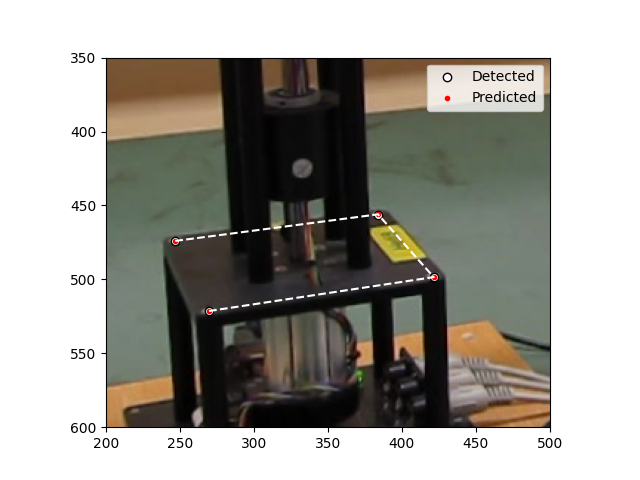
\includegraphics[width= 0.5 \linewidth]{../python/out_part2_2}
        \caption{Pose estimation with Levenberg-Marquardt}
    \end{figure*}

\section{Calibrate the model via batch optimization}
    \subsection*{Task 3.1}
    \begin{figure*}[h]
        \centering
        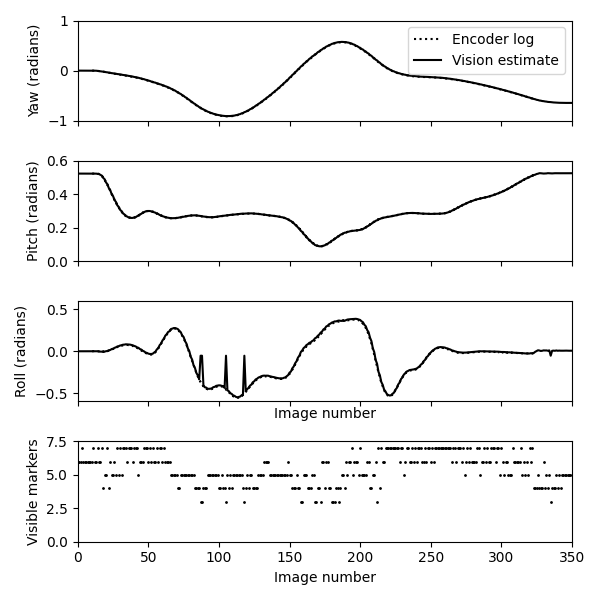
\includegraphics[width=0.5 \linewidth]{../python/out_part3_Mod-A}
        \caption{Plotted reprojection errors of the 3 angels and number of detected markers per image (model A)}
    \end{figure*}
    For model A we get the following reprojection errors: \\
    - Maximum: 1.1296 pixels\\
    - Average: 0.1690 pixels\\
    - Median: 0.1510 pixels\\
    30 iterations


        \begin{figure*}[h]
        \centering
        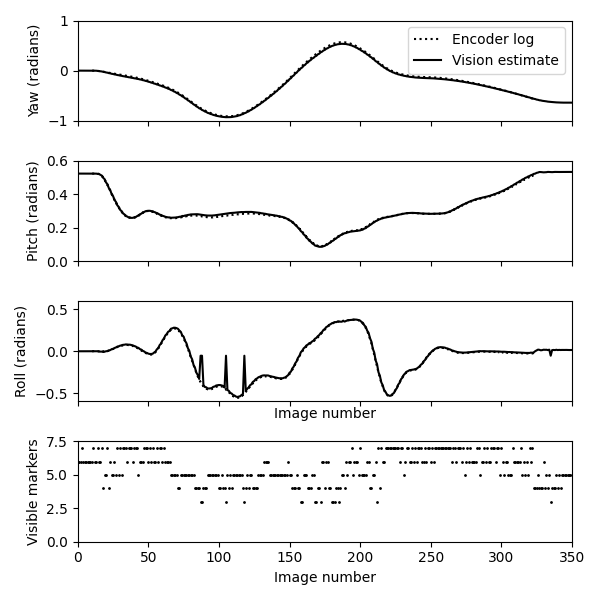
\includegraphics[width=0.5 \linewidth]{../python/out_part3_Mod-B}
        \caption{Plotted reprojection errors of the 3 angels and number of detected markers per image (modle B)}
    \end{figure*}
    For model A we get the following reprojection errors: \\
    - Maximum: 1.1199 pixels \\
    - Average: 0.1519 pixels \\
    - Median: 0.1328 pixels \\
    150 iterations

        \begin{figure*}[h]
        \centering
        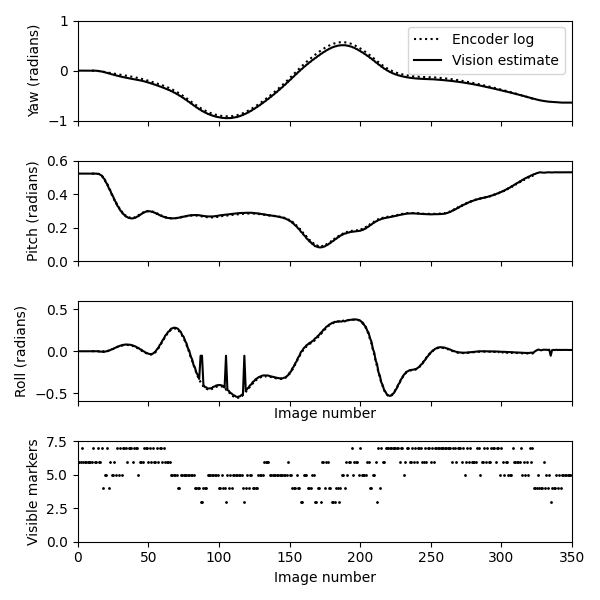
\includegraphics[width=0.5 \linewidth]{../python/out_part3_Mod-C}
        \caption{Plotted reprojection errors of the 3 angels and number of detected markers per image (model C)}
    \end{figure*}
    For model C we get the following reprojection errors: \\
    - Maximum: 1.1152 pixels\\
    - Average: 0.1525 pixels\\
    - Median: 0.1327 pixels \\
    600 iterations


    \subsection*{Task 3.2}
    As a standard starting point you can always try zero-initialisation what has proven to work well enough in many cases.
    But if this doesn't work you can always define a simpler model and use the best estimates of that as your new starting parameters.

    \subsection*{Task 3.3}
    No. If the '5cm length' had been 0, and the 32.5cm and 65cm ones were shorter, you could still end up with the same marker positions.


\end{document}
